\documentclass[hide notes,intlimits,usenames,dvipsnames]{beamer}

\mode<presentation>
{
  \usetheme{Singapore}
  \usefonttheme{professionalfonts}
  \setbeamertemplate{blocks}[rounded][shadow=true]
  \setbeamercovered{transparent}
  \setbeamertemplate{footline}[frame number]
}

% load packages
\usepackage[english]{babel}
\usepackage[latin1]{inputenc}
\usepackage[T1]{fontenc}
\usepackage{lmodern}
\usepackage[multidot]{grffile}
\usepackage{verbatim,empheq}

\usepackage{tikz}
\usetikzlibrary{shapes,arrows,shadows}
\usetikzlibrary{decorations.pathreplacing}

\usepackage{animate}
\usepackage{amsmath,verbatim}

% see http://tex.stackexchange.com/questions/86188/labelling-with-arrows-in-an-automated-way

\newif\ifclipme\clipmetrue
\tikzset{labelstyle/.style={LabelStyle/.append style={#1}},linestyle/.style={LineStyle/.append style={#1}}}
\tikzset{LabelStyle/.initial={},LineStyle/.initial={}}

\newcommand{\mathWithDescription}[4][]{{%
    \tikzset{#1}%
    \tikz[baseline]{
        \node[draw=red,rounded corners,anchor=base] (m#4) {$\displaystyle#2$};
        \ifclipme\begin{pgfinterruptboundingbox}\fi
            \node[above of=m#4,font=\strut, LabelStyle] (l#4) {#3};
            \draw[-,red, LineStyle] (l#4) to (m#4);
        \ifclipme\end{pgfinterruptboundingbox}\fi
    }%
}}

\newcommand{\mathWithDescriptionStarred}[3][]{{%
    \clipmefalse%
    \mathWithDescription[#1]{#2}{#3}{\themathLabelNode}%
}}

\newcounter{mathLabelNode}

\newcommand{\mathLabelBox}[3][]{%
   \stepcounter{mathLabelNode}%
   \mathWithDescription[#1]{#2}{#3}{\themathLabelNode}%
   \vphantom{\mathWithDescriptionStarred[#1]{#2}{#3}{\themathLabelNode}}%
}

\definecolor{dark red}{HTML}{E41A1C}
\definecolor{dark green}{HTML}{4DAF4A}
\definecolor{dark violet}{HTML}{984EA3}
\definecolor{dark blue}{HTML}{084594}
\definecolor{dark orange}{HTML}{FF7F00}
\definecolor{light blue}{HTML}{377EB8}
\definecolor{light red}{HTML}{FB9A99}
\definecolor{light violet}{HTML}{CAB2D6}

\newcommand{\CC}{\mathbb{C}}
\newcommand{\NN}{\mathbb{N}}
\newcommand{\RR}{\mathbb{R}}
\newcommand{\ZZ}{\mathbb{Z}}

\newcommand{\Kcal}{\mathcal{K}}
\newcommand{\Xcal}{\mathcal{X}}

\newcommand{\bF}{\mathbf{F}}
\newcommand{\bQ}{\mathbf{Q}}
\newcommand{\bU}{\mathbf{U}}
\newcommand{\bX}{\mathbf{X}}

\newcommand{\bb}{\mathbf{b}}
\newcommand{\bc}{\mathbf{c}}
\newcommand{\bn}{\mathbf{n}}
\newcommand{\bp}{\mathbf{p}}
\newcommand{\bq}{\mathbf{q}}
\newcommand{\bs}{\mathbf{s}}
\newcommand{\bu}{\mathbf{u}}
\newcommand{\bv}{\mathbf{v}}
\newcommand{\bx}{\mathbf{x}}

\newcommand{\Div}{\nabla\cdot}
\newcommand{\eps}{\epsilon}
\newcommand{\grad}{\nabla}
\newcommand{\lap}{\triangle}
\renewcommand{\bar}{\overline}

\newcommand{\ip}[2]{\ensuremath{\left<#1,#2\right>}}

\newcommand{\Span}{\operatorname{span}}

\newenvironment{transbox}[1][]{%
\begin{tikzpicture}
\node[drop shadow,rounded corners,text width=\textwidth,fill=white, fill opacity=#1,text opacity=1] \bgroup
}{
\egroup;\end{tikzpicture}}


\title{A practical view of the classical FEM}

\subtitle{(and some software)}

\author[Bueler]{Ed Bueler}

\institute[UAF]{
  \scriptsize Dept of Mathematics and Statistics \\

  University of Alaska Fairbanks
}

%\titlegraphic{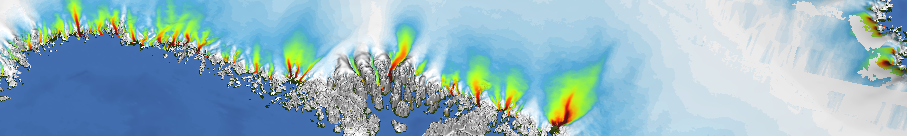
\includegraphics[width=\textwidth]{andycoast.png}}

\beamertemplatenavigationsymbolsempty   % remove faint and silly navigation symbols at bottom
\renewcommand{\insertnavigation}[1]{}   % remove section headings from top of each slide

\setbeamerfont{date}{size=\scriptsize}
\date{}

\AtBeginSection[]
{%
}


\begin{document}
\graphicspath{{figures/}}

\makeatletter
\providecommand*{\input@path}{}
\g@addto@macro\input@path{{tikz/}}% append;   \input@path is like \graphicspath
\makeatother


\begin{frame}
\vspace{10mm}
  \titlepage
  \begin{center}
  \tiny DMS \hfill 27 November 2018
  \end{center}
\end{frame}


\begin{frame}
    \frametitle{Outline}
    \tableofcontents
\end{frame}


\section{nonlinear Poisson problems with general boundary conditions}

\begin{frame}{general, nonlinear Poisson problem}
\begin{itemize}
\item $\Omega \subset \RR^2$ % with disjoint decomposition $\partial \Omega = \partial_D \Omega \cup \partial_N \Omega$
\item recall our usual problem: $\triangle u = f$, $u=0$ on $\partial\Omega$
\item these slides cover a nonlinear version with general boundary conditions:
\begin{align*}
- \Div \left(a(u) \grad u\right) &= f(u)  &&\text{ on } \Omega, \\
u &= g_D &&\text{ on } \partial_D \Omega, \notag \\
\frac{\partial u}{\partial n} &= g_N &&\text{ on } \partial_N \Omega. \notag
\end{align*}
\item $a(u,x,y)$, $f(u,x,y)$, $g_N(x,y)$, $g_D(x,y)$ are given (data)
\item nonlinear because $a=a(u)$ and/or $f=f(u)$ is allowed
%\item for well-posedness:
%    \begin{itemize}
%    \item[$\circ$] assume $a,f,g_N,g_D$ at least $L^2$ in $x,y$
%    \item[$\circ$] expect $f$ to be Lipschitz in $u$
%    \item[$\circ$] assume \emph{uniform ellipticity}: $a(u,x,y) \ge \eps > 0$
%    \end{itemize}
\end{itemize}
\end{frame}


\begin{frame}{general, nonlinear Poisson problem}
\begin{center}
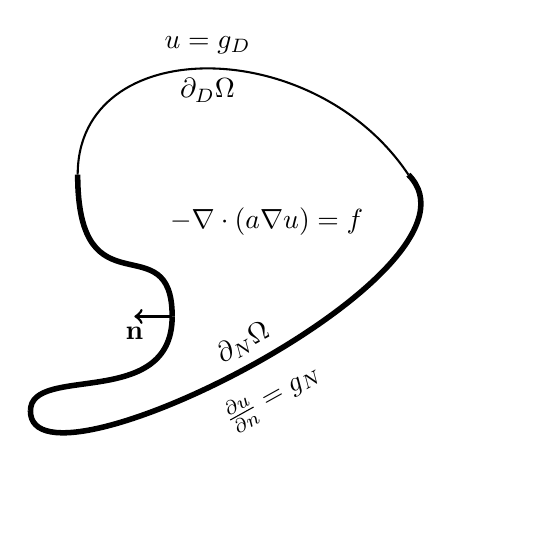
\begin{tikzpicture}[scale=0.6]
\draw[line width=0.75pt] (0,0) .. controls (0,3) and (5,3) .. node[sloped,above,yshift=0.5mm] {$u=g_D$} node[sloped,below] {$\partial_D\Omega$} (7,0);
\draw[line width=2pt] (7,0) .. controls (9,-2) and (-1,-7) .. node[sloped,above] {$\partial_N\Omega$} node[sloped,below,yshift=-1mm] {$\frac{\partial u}{\partial n} = g_N$} (-1,-5);
\draw[line width=2pt] (-1,-5) .. controls (-1,-4) and (2,-5) .. (2,-3);
\draw[line width=2pt] (2,-3) .. controls (2,-1) and (0,-3) .. (0,0);
\draw[->,line width=1.0pt] (2,-3) -- (1.2,-3) node[below] {$\bn$}; % normal vector
\draw (4,-1) node {$- \Div (a \grad u) = f$};
\end{tikzpicture}


\end{center}
\end{frame}


\begin{frame}{weak form}
\begin{itemize}
\item $u\in H_g^1(\Omega) = \{u\in H^1(\Omega)\,:\,u=g_D \text{ on } \partial_D\Omega\}$
    \begin{itemize}
    \item[$\circ$] Dirichlet data $g_D$ is used in defining $H^1_g(\Omega)$
    \end{itemize}
\item test functions: $H_0^1(\Omega) = \{v\in H^1(\Omega)\,:\,v=0 \text{ on } \partial_D\Omega\}$
\item for $v\in H^1_0(\Omega)$, multiply PDE by $v$ and integrate by parts:
\begin{equation*}
\int_\Omega a(u) \grad u \cdot \grad v - \int_{\partial\Omega} \frac{\partial u}{\partial n} v = \int_\Omega f(u) v
\end{equation*}
\item apply boundary conditions:
\begin{equation*}
\int_\Omega a(u) \grad u \cdot \grad v = \int_\Omega f(u) v + \int_{\partial_N\Omega} g_N v \tag{WF}
\end{equation*}

\vspace{-2mm}
    \begin{itemize}
    \item[$\circ$] Neumann data $g_N$ appears here
    \end{itemize}
\end{itemize}
\end{frame}


\begin{frame}{examples}
some examples of $- \Div \left(a(u) \grad u\right) = f(u)$:
\begin{itemize}
\item Poisson equation:
    $$-\triangle u=f(x,y), \quad u=0 \text{ on } \partial \Omega$$
\item Liouville-Bratu equation:
    $$-\triangle u = \lambda e^u$$

\vspace{-3mm}
    \begin{itemize}
    \item[$\circ$] critical $\lambda$ for well-posedness
    \end{itemize}
\item porous-medium equation:
    $$-\Div\left((u^{m-1} + \eps)\grad u\right) = f$$

\vspace{-3mm}
    \begin{itemize}
    \item[$\circ$] regularized with $\eps>0$ for uniform ellipticity
    \item[$\circ$] $\eps=0$: degeneracies within domain
    \end{itemize}
\end{itemize}
\end{frame}


\AtBeginSection[]
{
  \begin{frame}<beamer>
    \frametitle{Outline}
    %\tableofcontents[currentsection,hideallsubsections]
    \tableofcontents[currentsection]
  \end{frame}
}


\section{assembly of FEM system}

\begin{frame}{meshes and numbering}
\mbox{% created by command line:
%   tmp/petsc2tikz.py --labelelements --nodesize 1.0 --dirichletsize 3.0 --scale 0.63 tmp/blob1 -o tmp/blob1_elenum.tikz
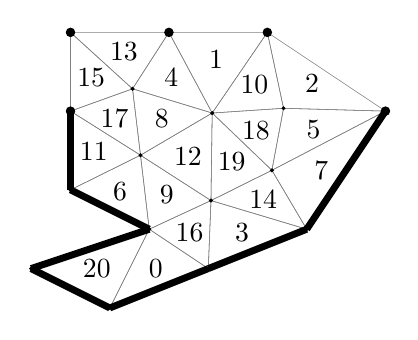
\begin{tikzpicture}[scale=0.5]
  \draw[gray,very thin] (2.000000,-3.000000) -- (3.500000,-4.000000) -- (1.000000,-5.000000) -- (2.000000,-3.000000) ;
  \draw (2.166667,-4.000000) node {$0$};
  \draw[gray,very thin] (5.000000,2.000000) -- (3.598633,-0.048909) -- (2.500000,2.000000) -- (5.000000,2.000000) ;
  \draw (3.699544,1.317030) node {$1$};
  \draw[gray,very thin] (5.000000,2.000000) -- (8.000000,0.000000) -- (5.410836,0.072145) -- (5.000000,2.000000) ;
  \draw (6.136945,0.690715) node {$2$};
  \draw[gray,very thin] (6.000000,-3.000000) -- (3.500000,-4.000000) -- (3.567839,-2.271643) -- (6.000000,-3.000000) ;
  \draw (4.355946,-3.090548) node {$3$};
  \draw[gray,very thin] (2.500000,2.000000) -- (3.598633,-0.048909) -- (1.575312,0.566253) -- (2.500000,2.000000) ;
  \draw (2.557982,0.839115) node {$4$};
  \draw[gray,very thin] (5.410836,0.072145) -- (8.000000,0.000000) -- (5.115191,-1.502985) -- (5.410836,0.072145) ;
  \draw (6.175342,-0.476947) node {$5$};
  \draw[gray,very thin] (2.000000,-3.000000) -- (0.000000,-2.000000) -- (1.777927,-1.119826) -- (2.000000,-3.000000) ;
  \draw (1.259309,-2.039942) node {$6$};
  \draw[gray,very thin] (8.000000,0.000000) -- (6.000000,-3.000000) -- (5.115191,-1.502985) -- (8.000000,0.000000) ;
  \draw (6.371730,-1.500995) node {$7$};
  \draw[gray,very thin] (3.598633,-0.048909) -- (1.777927,-1.119826) -- (1.575312,0.566253) -- (3.598633,-0.048909) ;
  \draw (2.317291,-0.200827) node {$8$};
  \draw[gray,very thin] (2.000000,-3.000000) -- (1.777927,-1.119826) -- (3.567839,-2.271643) -- (2.000000,-3.000000) ;
  \draw (2.448589,-2.130490) node {$9$};
  \draw[gray,very thin] (5.000000,2.000000) -- (5.410836,0.072145) -- (3.598633,-0.048909) -- (5.000000,2.000000) ;
  \draw (4.669823,0.674412) node {$10$};
  \draw[gray,very thin] (0.000000,0.000000) -- (1.777927,-1.119826) -- (0.000000,-2.000000) -- (0.000000,0.000000) ;
  \draw (0.592642,-1.039942) node {$11$};
  \draw[gray,very thin] (3.598633,-0.048909) -- (3.567839,-2.271643) -- (1.777927,-1.119826) -- (3.598633,-0.048909) ;
  \draw (2.981466,-1.146793) node {$12$};
  \draw[gray,very thin] (0.000000,2.000000) -- (2.500000,2.000000) -- (1.575312,0.566253) -- (0.000000,2.000000) ;
  \draw (1.358437,1.522084) node {$13$};
  \draw[gray,very thin] (6.000000,-3.000000) -- (3.567839,-2.271643) -- (5.115191,-1.502985) -- (6.000000,-3.000000) ;
  \draw (4.894343,-2.258209) node {$14$};
  \draw[gray,very thin] (0.000000,0.000000) -- (0.000000,2.000000) -- (1.575312,0.566253) -- (0.000000,0.000000) ;
  \draw (0.525104,0.855418) node {$15$};
  \draw[gray,very thin] (2.000000,-3.000000) -- (3.567839,-2.271643) -- (3.500000,-4.000000) -- (2.000000,-3.000000) ;
  \draw (3.022613,-3.090548) node {$16$};
  \draw[gray,very thin] (0.000000,0.000000) -- (1.575312,0.566253) -- (1.777927,-1.119826) -- (0.000000,0.000000) ;
  \draw (1.117746,-0.184524) node {$17$};
  \draw[gray,very thin] (3.598633,-0.048909) -- (5.410836,0.072145) -- (5.115191,-1.502985) -- (3.598633,-0.048909) ;
  \draw (4.708220,-0.493250) node {$18$};
  \draw[gray,very thin] (3.598633,-0.048909) -- (5.115191,-1.502985) -- (3.567839,-2.271643) -- (3.598633,-0.048909) ;
  \draw (4.093888,-1.274512) node {$19$};
  \draw[gray,very thin] (2.000000,-3.000000) -- (1.000000,-5.000000) -- (-1.000000,-4.000000) -- (2.000000,-3.000000) ;
  \draw (0.666667,-4.000000) node {$20$};
  \filldraw (0.000000,0.000000) circle (3.000000pt);
  \filldraw (0.000000,2.000000) circle (3.000000pt);
  \filldraw (5.000000,2.000000) circle (3.000000pt);
  \filldraw (8.000000,0.000000) circle (3.000000pt);
  \filldraw (6.000000,-3.000000) circle (1.000000pt);
  \filldraw (1.000000,-5.000000) circle (1.000000pt);
  \filldraw (-1.000000,-4.000000) circle (1.000000pt);
  \filldraw (2.000000,-3.000000) circle (1.000000pt);
  \filldraw (0.000000,-2.000000) circle (1.000000pt);
  \filldraw (2.500000,2.000000) circle (3.000000pt);
  \filldraw (3.500000,-4.000000) circle (1.000000pt);
  \filldraw (3.598633,-0.048909) circle (1.000000pt);
  \filldraw (1.777927,-1.119826) circle (1.000000pt);
  \filldraw (3.567839,-2.271643) circle (1.000000pt);
  \filldraw (5.410836,0.072145) circle (1.000000pt);
  \filldraw (1.575312,0.566253) circle (1.000000pt);
  \filldraw (5.115191,-1.502985) circle (1.000000pt);
  \draw[line width=2.500000pt] (8.000000,0.000000) -- (6.000000,-3.000000);
  \draw[line width=2.500000pt] (6.000000,-3.000000) -- (3.500000,-4.000000);
  \draw[line width=2.500000pt] (3.500000,-4.000000) -- (1.000000,-5.000000);
  \draw[line width=2.500000pt] (1.000000,-5.000000) -- (-1.000000,-4.000000);
  \draw[line width=2.500000pt] (-1.000000,-4.000000) -- (2.000000,-3.000000);
  \draw[line width=2.500000pt] (2.000000,-3.000000) -- (0.000000,-2.000000);
  \draw[line width=2.500000pt] (0.000000,-2.000000) -- (0.000000,0.000000);
\end{tikzpicture}
 \quad % created by command line:
%   tmp/petsc2tikz.py --labelnodes --nodesize 1.0 --dirichletsize 3.0 --nodeoffset -0.5 --scale 0.63 tmp/blob1 -o tmp/blob1_nodenum.tikz
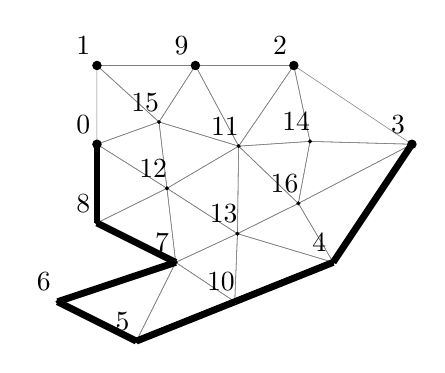
\begin{tikzpicture}[scale=0.5]
  \draw[gray,very thin] (2.000000,-3.000000) -- (3.500000,-4.000000) -- (1.000000,-5.000000) -- (2.000000,-3.000000) ;
  \draw[gray,very thin] (5.000000,2.000000) -- (3.598633,-0.048909) -- (2.500000,2.000000) -- (5.000000,2.000000) ;
  \draw[gray,very thin] (5.000000,2.000000) -- (8.000000,0.000000) -- (5.410836,0.072145) -- (5.000000,2.000000) ;
  \draw[gray,very thin] (6.000000,-3.000000) -- (3.500000,-4.000000) -- (3.567839,-2.271643) -- (6.000000,-3.000000) ;
  \draw[gray,very thin] (2.500000,2.000000) -- (3.598633,-0.048909) -- (1.575312,0.566253) -- (2.500000,2.000000) ;
  \draw[gray,very thin] (5.410836,0.072145) -- (8.000000,0.000000) -- (5.115191,-1.502985) -- (5.410836,0.072145) ;
  \draw[gray,very thin] (2.000000,-3.000000) -- (0.000000,-2.000000) -- (1.777927,-1.119826) -- (2.000000,-3.000000) ;
  \draw[gray,very thin] (8.000000,0.000000) -- (6.000000,-3.000000) -- (5.115191,-1.502985) -- (8.000000,0.000000) ;
  \draw[gray,very thin] (3.598633,-0.048909) -- (1.777927,-1.119826) -- (1.575312,0.566253) -- (3.598633,-0.048909) ;
  \draw[gray,very thin] (2.000000,-3.000000) -- (1.777927,-1.119826) -- (3.567839,-2.271643) -- (2.000000,-3.000000) ;
  \draw[gray,very thin] (5.000000,2.000000) -- (5.410836,0.072145) -- (3.598633,-0.048909) -- (5.000000,2.000000) ;
  \draw[gray,very thin] (0.000000,0.000000) -- (1.777927,-1.119826) -- (0.000000,-2.000000) -- (0.000000,0.000000) ;
  \draw[gray,very thin] (3.598633,-0.048909) -- (3.567839,-2.271643) -- (1.777927,-1.119826) -- (3.598633,-0.048909) ;
  \draw[gray,very thin] (0.000000,2.000000) -- (2.500000,2.000000) -- (1.575312,0.566253) -- (0.000000,2.000000) ;
  \draw[gray,very thin] (6.000000,-3.000000) -- (3.567839,-2.271643) -- (5.115191,-1.502985) -- (6.000000,-3.000000) ;
  \draw[gray,very thin] (0.000000,0.000000) -- (0.000000,2.000000) -- (1.575312,0.566253) -- (0.000000,0.000000) ;
  \draw[gray,very thin] (2.000000,-3.000000) -- (3.567839,-2.271643) -- (3.500000,-4.000000) -- (2.000000,-3.000000) ;
  \draw[gray,very thin] (0.000000,0.000000) -- (1.575312,0.566253) -- (1.777927,-1.119826) -- (0.000000,0.000000) ;
  \draw[gray,very thin] (3.598633,-0.048909) -- (5.410836,0.072145) -- (5.115191,-1.502985) -- (3.598633,-0.048909) ;
  \draw[gray,very thin] (3.598633,-0.048909) -- (5.115191,-1.502985) -- (3.567839,-2.271643) -- (3.598633,-0.048909) ;
  \draw[gray,very thin] (2.000000,-3.000000) -- (1.000000,-5.000000) -- (-1.000000,-4.000000) -- (2.000000,-3.000000) ;
  \filldraw (0.000000,0.000000) circle (3.000000pt);
  \draw (-0.350000,0.500000) node {$0$};
  \filldraw (0.000000,2.000000) circle (3.000000pt);
  \draw (-0.350000,2.500000) node {$1$};
  \filldraw (5.000000,2.000000) circle (3.000000pt);
  \draw (4.650000,2.500000) node {$2$};
  \filldraw (8.000000,0.000000) circle (3.000000pt);
  \draw (7.650000,0.500000) node {$3$};
  \filldraw (6.000000,-3.000000) circle (1.000000pt);
  \draw (5.650000,-2.500000) node {$4$};
  \filldraw (1.000000,-5.000000) circle (1.000000pt);
  \draw (0.650000,-4.500000) node {$5$};
  \filldraw (-1.000000,-4.000000) circle (1.000000pt);
  \draw (-1.350000,-3.500000) node {$6$};
  \filldraw (2.000000,-3.000000) circle (1.000000pt);
  \draw (1.650000,-2.500000) node {$7$};
  \filldraw (0.000000,-2.000000) circle (1.000000pt);
  \draw (-0.350000,-1.500000) node {$8$};
  \filldraw (2.500000,2.000000) circle (3.000000pt);
  \draw (2.150000,2.500000) node {$9$};
  \filldraw (3.500000,-4.000000) circle (1.000000pt);
  \draw (3.150000,-3.500000) node {$10$};
  \filldraw (3.598633,-0.048909) circle (1.000000pt);
  \draw (3.248633,0.451091) node {$11$};
  \filldraw (1.777927,-1.119826) circle (1.000000pt);
  \draw (1.427927,-0.619826) node {$12$};
  \filldraw (3.567839,-2.271643) circle (1.000000pt);
  \draw (3.217839,-1.771643) node {$13$};
  \filldraw (5.410836,0.072145) circle (1.000000pt);
  \draw (5.060836,0.572145) node {$14$};
  \filldraw (1.575312,0.566253) circle (1.000000pt);
  \draw (1.225312,1.066253) node {$15$};
  \filldraw (5.115191,-1.502985) circle (1.000000pt);
  \draw (4.765191,-1.002985) node {$16$};
  \draw[line width=2.500000pt] (8.000000,0.000000) -- (6.000000,-3.000000);
  \draw[line width=2.500000pt] (6.000000,-3.000000) -- (3.500000,-4.000000);
  \draw[line width=2.500000pt] (3.500000,-4.000000) -- (1.000000,-5.000000);
  \draw[line width=2.500000pt] (1.000000,-5.000000) -- (-1.000000,-4.000000);
  \draw[line width=2.500000pt] (-1.000000,-4.000000) -- (2.000000,-3.000000);
  \draw[line width=2.500000pt] (2.000000,-3.000000) -- (0.000000,-2.000000);
  \draw[line width=2.500000pt] (0.000000,-2.000000) -- (0.000000,0.000000);
\end{tikzpicture}
}

\begin{itemize}
\item triangulation $\mathcal{T}_h$ of a polygonal domain $\Omega$
\item numbering:
    \begin{itemize}
    \item[$\circ$] $K$ elements ($=21$ above; left)
    \item[$\circ$] $N$ nodes ($=17$ above; right)
    \item[$\circ$] $P$ segments in Neumann boundary ($=7$ above; bold)
    \item[$\circ$] $n_D$ nodes in Dirichlet boundary ($=5$ above)
    \end{itemize}
\item to fully describe mesh, also need node locations $\bx_i=(x_i,y_i)$
\end{itemize}
\end{frame}


\begin{frame}{FEM spaces}
\vspace{4mm}

\begin{itemize}
\item hat functions satisfy:
    \begin{itemize}
    \item[$\circ$] $\psi_j(\bx)$ continuous
    \item[$\circ$] $\psi_j \in P_1$ on each element
    \item[$\circ$] $\psi_j(\bx_i)=\delta_{ij}$
    \end{itemize}

\vspace{-19mm}

\hfill     % (2,2,1) is top
    \draw (0,0,0) -- (2,2,1); % to top from left
    \draw (4,0,0) -- (2,2,1); %   ...  from front
    \draw (4,0,3) -- (2,2,1); %   ...  from right
    \draw[color=gray] (0.3,0,4) -- (2,2,1); % from back
    \draw[color=gray] (2,0.4,1) -- (2,2,1); % from middle

    % draw base
    \draw (0,0,0) -- (4,0,0);
    \draw (4,0,0) -- (4,0,3);
    \draw[color=gray] (0,0,0) -- (0.3,0,4);
    \draw[color=gray] (0.3,0,4) -- (4,0,3);
    \draw[color=gray] (0,0,0) -- (2,0.4,1);
    \draw[color=gray] (2,0.4,1) -- (4,0,3);
    \draw[color=gray] (4,0,0) -- (2,0.4,1);
    \draw[color=gray] (2,0.4,1) -- (0.3,0,4);

    % extend flat
    \draw (0,0,0) -- (-0.7,-0.7,0);
    \draw (0,0,0) -- (1.5,-0.6,0);
    \draw (0,0,0) -- (-1,0.6,0);
    \draw (4,0,0) -- (1.5,-0.6,0);
    \draw (4,0,0) -- (5.5,0.1,0);
    \draw (4,0,0) -- (5,-0.5,0);
    \draw (4,0,3) -- (5.5,0.1,0);
    \draw (4,0,3) -- (5,0,2);

    % label node j
    \draw (2,2,1.9) node {{\scriptsize $\psi_j=1$}};
    \draw (2,0.15,0.8) node {{\scriptsize node $j$}};
    \draw (2,0.4,1) circle (4.0pt);

    % draw nodes
    \filldraw[color=gray] (0.3,0,4) circle (0.8pt);
    \filldraw[color=gray] (2,0.4,1) circle (1.0pt);
    \filldraw (4,0,3) circle (1.0pt);
    \filldraw (0,0,0) circle (1.25pt);
    \filldraw (4,0,0) circle (1.25pt);
    \filldraw (5.5,0.1,0) circle (1.25pt);
    \filldraw (1.5,-0.6,0) circle (1.5pt);

\item use hat functions to approximate $g_D(\bx)$:
\begin{equation*}
\hat g_D(\bx) = \sum_{l=0}^{n_D-1} g_D(\bx_{j_l}) \psi_{j_l}(\bx) \quad \in C(\overline\Omega)
\end{equation*}
\item use hat functions to define test function space:
\begin{equation*}
S_{0}^h = \Span\left<\psi_j \,:\, \bx_j \notin \partial_D \Omega\right> \subset H_0^1(\Omega)
\end{equation*}
\item \dots and trial function space:
\begin{equation*}
S_{g}^h = \left\{\hat g_D + w \,:\, w \in S_{0}^h\right\} \stackrel{?}{\subset} H_g^1(\Omega)
\end{equation*}
\end{itemize}
\end{frame}


\begin{frame}{FEM spaces}
\begin{itemize}
\item expand the FEM solution $u^h$:
\begin{equation*}
u^h(\bx) = \hat g_D(\bx) + \sum_{\bx_j \notin \partial_D \Omega} u_j\, \psi_j(\bx)
\end{equation*}
\item discrete weak form:  for all $i$ such that $\bx_i \notin \partial_D \Omega$,
\begin{equation*}
\int_\Omega a(u^h) \grad u^h \cdot \grad \psi_i = \int_\Omega f(u^h) \psi_i + \int_{\partial_N\Omega} g_N \psi_i  \tag{DWF}
\end{equation*}
\item $\dim(S_{0}^h)=\dim(S_{g}^h)=N-n_D$
\item however, it is easier to also make Dirichlet boundary nodes into degrees of freedom
    \begin{itemize}
    \item[$\circ$] we assemble a nonlinear system of $N$ equations in $N$ unknowns
    \end{itemize}
\end{itemize}
\end{frame}


\begin{frame}{element residuals}
\begin{itemize}
\item for each element $\triangle_k$ and $\psi_i$, define an \emph{element residual}:
\begin{equation*}
F_i^k(\bu) = \int_{\triangle_k} a(u^h) \grad u^h \cdot \grad \psi_i - f(u^h) \psi_i
\end{equation*}
\item for each edge $s_\nu$ in the Neumann boundary we define
\begin{equation*}
\varphi_i^\nu = \int_{s_\nu} g_N \psi_i
\end{equation*}

\vspace{-2mm}
\item (DWF) becomes:
\begin{equation*}
F_i(\bu) = \sum_{k=0}^{K-1} F_i^k(\bu) - \sum_{\nu=0}^{P-1} \varphi_i^\nu = 0 \qquad \text{ for } \bx_i \notin \partial_D\Omega
\end{equation*}
\item for Dirichlet boundary nodes have easy equation:
\begin{equation*}
F_i(\bu) = u_i - g_D(\bx_i) \qquad \text{ for } \bx_i \in \partial_D\Omega
\end{equation*}
\end{itemize}
\end{frame}


\begin{frame}{assembled FEM system of equations}
\begin{itemize}
\item recall: $N$ is number of nodes in mesh
\item $P^1$ FEM generates an algebraic system of $N$ equations in $N$ unknowns:
\begin{equation*}
\bF(\bu)=0  \tag{$\ast$}
\end{equation*}
    \begin{itemize}
    \item[$\circ$] one equation $F_i(\bu)=0$ per node
    \item[$\circ$] one unknown $u_i$ per node
    \item[$\circ$] nonlinear system if $\partial a/\partial u \ne 0$ and/or $\partial f/\partial u \ne 0$
    \item[$\circ$] sparse because support of a hat function $\psi_i$ only overlaps with a few triangles $\triangle_k$, and thus only a few nodal values $\bu=\{u_j\}$ enter into a given $F_i^k(\bu)$
    \item[$\circ$] $J_{\bF} = (\partial \bF_i/\partial u_j)$ is the \emph{Jacobian}, a sparse matrix
    \end{itemize}
\end{itemize}
\end{frame}


\section{solving the equations}

\begin{frame}{nonlinear residual}
\begin{itemize}
\item the result of FEM assembly is a nonlinear system:
\begin{equation*}
\bF(\bu)=0  \tag{$\ast$}
\end{equation*}
\item the function $\bF:\RR^N \to \RR^N$ is called the  \emph{residual}
    \begin{itemize}
    \item[$\circ$] continuous and differentiable if $a,f$ are
    \end{itemize}
\item propose to solve ($\ast$) by Newton method:
\begin{align*}
    J_\bF(\bu_k) \bp &= - \bF(\bu_k)  \\
    \bu_{k+1} &= \bu_k + \alpha \bp
\end{align*}

\vspace{-2mm}
    \begin{itemize}
    \item[$\circ$] find $\alpha$ using line search based on \emph{merit function} $\Phi(\bu)=\frac{1}{2}\|\bF(\bu)\|^2$
    \item[$\circ$] converges in one step if $a=a(x,y)$ and $f=f(x,y)$ [linear]
    \item[$\circ$] converges quadratically if $a$, $f$ smooth
    \end{itemize}
\end{itemize}
\end{frame}


\begin{frame}{the Jacobian is the FEM stiffness matrix}
\begin{itemize}
\item $J_\bF(\bu)$ is the FEM ``stiffness matrix''
\item example: meshes with $N=7,18,55$ nodes

\bigskip
% created by command line:
%   tmp/petsc2tikz.py --nodesize 0.3 --dirichletsize 0.8 --neumannwidth 1.5 --scale 2.5 tmp/trap1 -o tmp/trap1.tikz
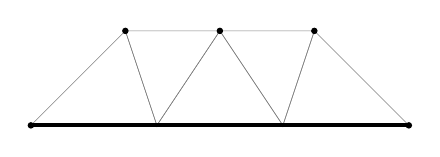
\begin{tikzpicture}[scale=1.200000]
  \draw[gray,very thin] (0.666667,0.000000) -- (0.000000,1.000000) -- (-0.666667,0.000000) -- (0.666667,0.000000) ;
  \draw[gray,very thin] (0.666667,0.000000) -- (2.000000,0.000000) -- (1.000000,1.000000) -- (0.666667,0.000000) ;
  \draw[gray,very thin] (-2.000000,0.000000) -- (-0.666667,0.000000) -- (-1.000000,1.000000) -- (-2.000000,0.000000) ;
  \draw[gray,very thin] (-0.666667,0.000000) -- (0.000000,1.000000) -- (-1.000000,1.000000) -- (-0.666667,0.000000) ;
  \draw[gray,very thin] (0.666667,0.000000) -- (1.000000,1.000000) -- (0.000000,1.000000) -- (0.666667,0.000000) ;
  \filldraw (2.000000,0.000000) circle (0.800000pt);
  \filldraw (1.000000,1.000000) circle (0.800000pt);
  \filldraw (-1.000000,1.000000) circle (0.800000pt);
  \filldraw (-2.000000,0.000000) circle (0.800000pt);
  \filldraw (0.000000,1.000000) circle (0.800000pt);
  \filldraw (-0.666667,0.000000) circle (0.300000pt);
  \filldraw (0.666667,0.000000) circle (0.300000pt);
  \draw[line width=1.500000pt] (-2.000000,0.000000) -- (-0.666667,0.000000);
  \draw[line width=1.500000pt] (-0.666667,0.000000) -- (0.666667,0.000000);
  \draw[line width=1.500000pt] (0.666667,0.000000) -- (2.000000,0.000000);
\end{tikzpicture}
 \hfill % created by command line:
%   tmp/petsc2tikz.py --nodesize 0.3 --dirichletsize 0.8 --neumannwidth 1.5 --scale 1.5 tmp/traps -o tmp/traps.tikz
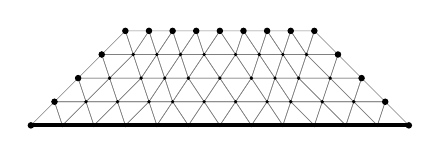
\begin{tikzpicture}[scale=1.200000]
  \draw[gray,very thin] (0.666667,0.000000) -- (0.500000,0.250000) -- (0.333333,0.000000) -- (0.666667,0.000000) ;
  \draw[gray,very thin] (0.500000,0.250000) -- (0.166667,0.250000) -- (0.333333,0.000000) -- (0.500000,0.250000) ;
  \draw[gray,very thin] (0.500000,0.250000) -- (0.333333,0.500000) -- (0.166667,0.250000) -- (0.500000,0.250000) ;
  \draw[gray,very thin] (0.333333,0.000000) -- (0.166667,0.250000) -- (-0.000000,0.000000) -- (0.333333,0.000000) ;
  \draw[gray,very thin] (0.333333,0.500000) -- (-0.000000,0.500000) -- (0.166667,0.250000) -- (0.333333,0.500000) ;
  \draw[gray,very thin] (-0.000000,0.500000) -- (-0.166667,0.250000) -- (0.166667,0.250000) -- (-0.000000,0.500000) ;
  \draw[gray,very thin] (-0.000000,0.500000) -- (-0.333333,0.500000) -- (-0.166667,0.250000) -- (-0.000000,0.500000) ;
  \draw[gray,very thin] (0.166667,0.250000) -- (-0.166667,0.250000) -- (-0.000000,0.000000) -- (0.166667,0.250000) ;
  \draw[gray,very thin] (0.333333,0.500000) -- (0.166667,0.750000) -- (-0.000000,0.500000) -- (0.333333,0.500000) ;
  \draw[gray,very thin] (0.166667,0.750000) -- (-0.166667,0.750000) -- (-0.000000,0.500000) -- (0.166667,0.750000) ;
  \draw[gray,very thin] (0.166667,0.750000) -- (0.000000,1.000000) -- (-0.166667,0.750000) -- (0.166667,0.750000) ;
  \draw[gray,very thin] (-0.000000,0.500000) -- (-0.166667,0.750000) -- (-0.333333,0.500000) -- (-0.000000,0.500000) ;
  \draw[gray,very thin] (-0.000000,0.000000) -- (-0.166667,0.250000) -- (-0.333333,0.000000) -- (-0.000000,0.000000) ;
  \draw[gray,very thin] (-0.166667,0.250000) -- (-0.500000,0.250000) -- (-0.333333,0.000000) -- (-0.166667,0.250000) ;
  \draw[gray,very thin] (-0.166667,0.250000) -- (-0.333333,0.500000) -- (-0.500000,0.250000) -- (-0.166667,0.250000) ;
  \draw[gray,very thin] (-0.333333,0.000000) -- (-0.500000,0.250000) -- (-0.666667,0.000000) -- (-0.333333,0.000000) ;
  \draw[gray,very thin] (0.666667,0.000000) -- (1.000000,0.000000) -- (0.750000,0.250000) -- (0.666667,0.000000) ;
  \draw[gray,very thin] (1.000000,0.000000) -- (1.083333,0.250000) -- (0.750000,0.250000) -- (1.000000,0.000000) ;
  \draw[gray,very thin] (1.000000,0.000000) -- (1.333333,0.000000) -- (1.083333,0.250000) -- (1.000000,0.000000) ;
  \draw[gray,very thin] (0.750000,0.250000) -- (1.083333,0.250000) -- (0.833333,0.500000) -- (0.750000,0.250000) ;
  \draw[gray,very thin] (1.333333,0.000000) -- (1.416667,0.250000) -- (1.083333,0.250000) -- (1.333333,0.000000) ;
  \draw[gray,very thin] (1.416667,0.250000) -- (1.166667,0.500000) -- (1.083333,0.250000) -- (1.416667,0.250000) ;
  \draw[gray,very thin] (1.416667,0.250000) -- (1.500000,0.500000) -- (1.166667,0.500000) -- (1.416667,0.250000) ;
  \draw[gray,very thin] (1.083333,0.250000) -- (1.166667,0.500000) -- (0.833333,0.500000) -- (1.083333,0.250000) ;
  \draw[gray,very thin] (1.333333,0.000000) -- (1.666667,0.000000) -- (1.416667,0.250000) -- (1.333333,0.000000) ;
  \draw[gray,very thin] (1.666667,0.000000) -- (1.750000,0.250000) -- (1.416667,0.250000) -- (1.666667,0.000000) ;
  \draw[gray,very thin] (1.666667,0.000000) -- (2.000000,0.000000) -- (1.750000,0.250000) -- (1.666667,0.000000) ;
  \draw[gray,very thin] (1.416667,0.250000) -- (1.750000,0.250000) -- (1.500000,0.500000) -- (1.416667,0.250000) ;
  \draw[gray,very thin] (0.833333,0.500000) -- (1.166667,0.500000) -- (0.916667,0.750000) -- (0.833333,0.500000) ;
  \draw[gray,very thin] (1.166667,0.500000) -- (1.250000,0.750000) -- (0.916667,0.750000) -- (1.166667,0.500000) ;
  \draw[gray,very thin] (1.166667,0.500000) -- (1.500000,0.500000) -- (1.250000,0.750000) -- (1.166667,0.500000) ;
  \draw[gray,very thin] (0.916667,0.750000) -- (1.250000,0.750000) -- (1.000000,1.000000) -- (0.916667,0.750000) ;
  \draw[gray,very thin] (-2.000000,0.000000) -- (-1.666667,0.000000) -- (-1.750000,0.250000) -- (-2.000000,0.000000) ;
  \draw[gray,very thin] (-1.666667,0.000000) -- (-1.416667,0.250000) -- (-1.750000,0.250000) -- (-1.666667,0.000000) ;
  \draw[gray,very thin] (-1.666667,0.000000) -- (-1.333333,0.000000) -- (-1.416667,0.250000) -- (-1.666667,0.000000) ;
  \draw[gray,very thin] (-1.750000,0.250000) -- (-1.416667,0.250000) -- (-1.500000,0.500000) -- (-1.750000,0.250000) ;
  \draw[gray,very thin] (-1.333333,0.000000) -- (-1.083333,0.250000) -- (-1.416667,0.250000) -- (-1.333333,0.000000) ;
  \draw[gray,very thin] (-1.083333,0.250000) -- (-1.166667,0.500000) -- (-1.416667,0.250000) -- (-1.083333,0.250000) ;
  \draw[gray,very thin] (-1.083333,0.250000) -- (-0.833333,0.500000) -- (-1.166667,0.500000) -- (-1.083333,0.250000) ;
  \draw[gray,very thin] (-1.416667,0.250000) -- (-1.166667,0.500000) -- (-1.500000,0.500000) -- (-1.416667,0.250000) ;
  \draw[gray,very thin] (-1.333333,0.000000) -- (-1.000000,0.000000) -- (-1.083333,0.250000) -- (-1.333333,0.000000) ;
  \draw[gray,very thin] (-1.000000,0.000000) -- (-0.750000,0.250000) -- (-1.083333,0.250000) -- (-1.000000,0.000000) ;
  \draw[gray,very thin] (-1.000000,0.000000) -- (-0.666667,0.000000) -- (-0.750000,0.250000) -- (-1.000000,0.000000) ;
  \draw[gray,very thin] (-1.083333,0.250000) -- (-0.750000,0.250000) -- (-0.833333,0.500000) -- (-1.083333,0.250000) ;
  \draw[gray,very thin] (-1.500000,0.500000) -- (-1.166667,0.500000) -- (-1.250000,0.750000) -- (-1.500000,0.500000) ;
  \draw[gray,very thin] (-1.166667,0.500000) -- (-0.916667,0.750000) -- (-1.250000,0.750000) -- (-1.166667,0.500000) ;
  \draw[gray,very thin] (-1.166667,0.500000) -- (-0.833333,0.500000) -- (-0.916667,0.750000) -- (-1.166667,0.500000) ;
  \draw[gray,very thin] (-1.250000,0.750000) -- (-0.916667,0.750000) -- (-1.000000,1.000000) -- (-1.250000,0.750000) ;
  \draw[gray,very thin] (-0.666667,0.000000) -- (-0.500000,0.250000) -- (-0.750000,0.250000) -- (-0.666667,0.000000) ;
  \draw[gray,very thin] (-0.500000,0.250000) -- (-0.583333,0.500000) -- (-0.750000,0.250000) -- (-0.500000,0.250000) ;
  \draw[gray,very thin] (-0.500000,0.250000) -- (-0.333333,0.500000) -- (-0.583333,0.500000) -- (-0.500000,0.250000) ;
  \draw[gray,very thin] (-0.750000,0.250000) -- (-0.583333,0.500000) -- (-0.833333,0.500000) -- (-0.750000,0.250000) ;
  \draw[gray,very thin] (-0.333333,0.500000) -- (-0.416667,0.750000) -- (-0.583333,0.500000) -- (-0.333333,0.500000) ;
  \draw[gray,very thin] (-0.416667,0.750000) -- (-0.666667,0.750000) -- (-0.583333,0.500000) -- (-0.416667,0.750000) ;
  \draw[gray,very thin] (-0.416667,0.750000) -- (-0.500000,1.000000) -- (-0.666667,0.750000) -- (-0.416667,0.750000) ;
  \draw[gray,very thin] (-0.583333,0.500000) -- (-0.666667,0.750000) -- (-0.833333,0.500000) -- (-0.583333,0.500000) ;
  \draw[gray,very thin] (-0.333333,0.500000) -- (-0.166667,0.750000) -- (-0.416667,0.750000) -- (-0.333333,0.500000) ;
  \draw[gray,very thin] (-0.166667,0.750000) -- (-0.250000,1.000000) -- (-0.416667,0.750000) -- (-0.166667,0.750000) ;
  \draw[gray,very thin] (-0.166667,0.750000) -- (0.000000,1.000000) -- (-0.250000,1.000000) -- (-0.166667,0.750000) ;
  \draw[gray,very thin] (-0.416667,0.750000) -- (-0.250000,1.000000) -- (-0.500000,1.000000) -- (-0.416667,0.750000) ;
  \draw[gray,very thin] (-0.833333,0.500000) -- (-0.666667,0.750000) -- (-0.916667,0.750000) -- (-0.833333,0.500000) ;
  \draw[gray,very thin] (-0.666667,0.750000) -- (-0.750000,1.000000) -- (-0.916667,0.750000) -- (-0.666667,0.750000) ;
  \draw[gray,very thin] (-0.666667,0.750000) -- (-0.500000,1.000000) -- (-0.750000,1.000000) -- (-0.666667,0.750000) ;
  \draw[gray,very thin] (-0.916667,0.750000) -- (-0.750000,1.000000) -- (-1.000000,1.000000) -- (-0.916667,0.750000) ;
  \draw[gray,very thin] (0.666667,0.000000) -- (0.750000,0.250000) -- (0.500000,0.250000) -- (0.666667,0.000000) ;
  \draw[gray,very thin] (0.750000,0.250000) -- (0.583333,0.500000) -- (0.500000,0.250000) -- (0.750000,0.250000) ;
  \draw[gray,very thin] (0.750000,0.250000) -- (0.833333,0.500000) -- (0.583333,0.500000) -- (0.750000,0.250000) ;
  \draw[gray,very thin] (0.500000,0.250000) -- (0.583333,0.500000) -- (0.333333,0.500000) -- (0.500000,0.250000) ;
  \draw[gray,very thin] (0.833333,0.500000) -- (0.666667,0.750000) -- (0.583333,0.500000) -- (0.833333,0.500000) ;
  \draw[gray,very thin] (0.666667,0.750000) -- (0.416667,0.750000) -- (0.583333,0.500000) -- (0.666667,0.750000) ;
  \draw[gray,very thin] (0.666667,0.750000) -- (0.500000,1.000000) -- (0.416667,0.750000) -- (0.666667,0.750000) ;
  \draw[gray,very thin] (0.583333,0.500000) -- (0.416667,0.750000) -- (0.333333,0.500000) -- (0.583333,0.500000) ;
  \draw[gray,very thin] (0.833333,0.500000) -- (0.916667,0.750000) -- (0.666667,0.750000) -- (0.833333,0.500000) ;
  \draw[gray,very thin] (0.916667,0.750000) -- (0.750000,1.000000) -- (0.666667,0.750000) -- (0.916667,0.750000) ;
  \draw[gray,very thin] (0.916667,0.750000) -- (1.000000,1.000000) -- (0.750000,1.000000) -- (0.916667,0.750000) ;
  \draw[gray,very thin] (0.666667,0.750000) -- (0.750000,1.000000) -- (0.500000,1.000000) -- (0.666667,0.750000) ;
  \draw[gray,very thin] (0.333333,0.500000) -- (0.416667,0.750000) -- (0.166667,0.750000) -- (0.333333,0.500000) ;
  \draw[gray,very thin] (0.416667,0.750000) -- (0.250000,1.000000) -- (0.166667,0.750000) -- (0.416667,0.750000) ;
  \draw[gray,very thin] (0.416667,0.750000) -- (0.500000,1.000000) -- (0.250000,1.000000) -- (0.416667,0.750000) ;
  \draw[gray,very thin] (0.166667,0.750000) -- (0.250000,1.000000) -- (0.000000,1.000000) -- (0.166667,0.750000) ;
  \filldraw (2.000000,0.000000) circle (0.800000pt);
  \filldraw (1.000000,1.000000) circle (0.800000pt);
  \filldraw (1.500000,0.500000) circle (0.800000pt);
  \filldraw (1.750000,0.250000) circle (0.800000pt);
  \filldraw (1.250000,0.750000) circle (0.800000pt);
  \filldraw (-1.000000,1.000000) circle (0.800000pt);
  \filldraw (0.000000,1.000000) circle (0.800000pt);
  \filldraw (0.500000,1.000000) circle (0.800000pt);
  \filldraw (-0.500000,1.000000) circle (0.800000pt);
  \filldraw (0.750000,1.000000) circle (0.800000pt);
  \filldraw (0.250000,1.000000) circle (0.800000pt);
  \filldraw (-0.250000,1.000000) circle (0.800000pt);
  \filldraw (-0.750000,1.000000) circle (0.800000pt);
  \filldraw (-2.000000,0.000000) circle (0.800000pt);
  \filldraw (-1.500000,0.500000) circle (0.800000pt);
  \filldraw (-1.250000,0.750000) circle (0.800000pt);
  \filldraw (-1.750000,0.250000) circle (0.800000pt);
  \filldraw (-0.666667,0.000000) circle (0.300000pt);
  \filldraw (0.666667,0.000000) circle (0.300000pt);
  \filldraw (-1.333333,0.000000) circle (0.300000pt);
  \filldraw (-0.000000,0.000000) circle (0.300000pt);
  \filldraw (1.333333,0.000000) circle (0.300000pt);
  \filldraw (-1.666667,0.000000) circle (0.300000pt);
  \filldraw (-1.000000,0.000000) circle (0.300000pt);
  \filldraw (-0.333333,0.000000) circle (0.300000pt);
  \filldraw (0.333333,0.000000) circle (0.300000pt);
  \filldraw (1.000000,0.000000) circle (0.300000pt);
  \filldraw (1.666667,0.000000) circle (0.300000pt);
  \filldraw (0.333333,0.500000) circle (0.300000pt);
  \filldraw (-0.333333,0.500000) circle (0.300000pt);
  \filldraw (0.833333,0.500000) circle (0.300000pt);
  \filldraw (-0.833333,0.500000) circle (0.300000pt);
  \filldraw (0.500000,0.250000) circle (0.300000pt);
  \filldraw (0.166667,0.250000) circle (0.300000pt);
  \filldraw (-0.000000,0.500000) circle (0.300000pt);
  \filldraw (-0.166667,0.250000) circle (0.300000pt);
  \filldraw (0.166667,0.750000) circle (0.300000pt);
  \filldraw (-0.166667,0.750000) circle (0.300000pt);
  \filldraw (-0.500000,0.250000) circle (0.300000pt);
  \filldraw (1.083333,0.250000) circle (0.300000pt);
  \filldraw (0.750000,0.250000) circle (0.300000pt);
  \filldraw (1.416667,0.250000) circle (0.300000pt);
  \filldraw (1.166667,0.500000) circle (0.300000pt);
  \filldraw (0.916667,0.750000) circle (0.300000pt);
  \filldraw (-1.416667,0.250000) circle (0.300000pt);
  \filldraw (-1.083333,0.250000) circle (0.300000pt);
  \filldraw (-1.166667,0.500000) circle (0.300000pt);
  \filldraw (-0.750000,0.250000) circle (0.300000pt);
  \filldraw (-0.916667,0.750000) circle (0.300000pt);
  \filldraw (-0.583333,0.500000) circle (0.300000pt);
  \filldraw (-0.416667,0.750000) circle (0.300000pt);
  \filldraw (-0.666667,0.750000) circle (0.300000pt);
  \filldraw (0.583333,0.500000) circle (0.300000pt);
  \filldraw (0.666667,0.750000) circle (0.300000pt);
  \filldraw (0.416667,0.750000) circle (0.300000pt);
  \draw[line width=1.500000pt] (-2.000000,0.000000) -- (-1.666667,0.000000);
  \draw[line width=1.500000pt] (-1.666667,0.000000) -- (-1.333333,0.000000);
  \draw[line width=1.500000pt] (-1.333333,0.000000) -- (-1.000000,0.000000);
  \draw[line width=1.500000pt] (-1.000000,0.000000) -- (-0.666667,0.000000);
  \draw[line width=1.500000pt] (-0.666667,0.000000) -- (-0.333333,0.000000);
  \draw[line width=1.500000pt] (-0.333333,0.000000) -- (-0.000000,0.000000);
  \draw[line width=1.500000pt] (-0.000000,0.000000) -- (0.333333,0.000000);
  \draw[line width=1.500000pt] (0.333333,0.000000) -- (0.666667,0.000000);
  \draw[line width=1.500000pt] (0.666667,0.000000) -- (1.000000,0.000000);
  \draw[line width=1.500000pt] (1.000000,0.000000) -- (1.333333,0.000000);
  \draw[line width=1.500000pt] (1.333333,0.000000) -- (1.666667,0.000000);
  \draw[line width=1.500000pt] (1.666667,0.000000) -- (2.000000,0.000000);
\end{tikzpicture}


\vspace{-2mm}
    \begin{itemize}
    \item[$\circ$] generated by uniform refinement of $N=7$ mesh
    \item[$\circ$] $N=18$ mesh not shown
    \end{itemize}
\item sparsity patterns for corresponding $J_\bF(\bu)$:

\bigskip\bigskip
\mbox{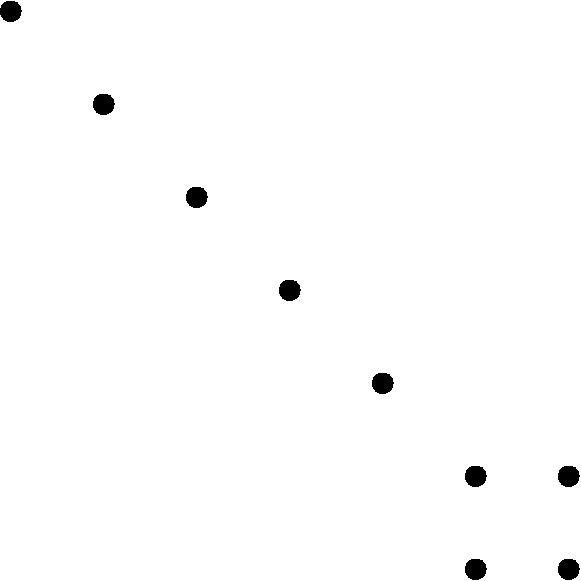
\includegraphics[width=0.25\textwidth]{trap1mat} \, 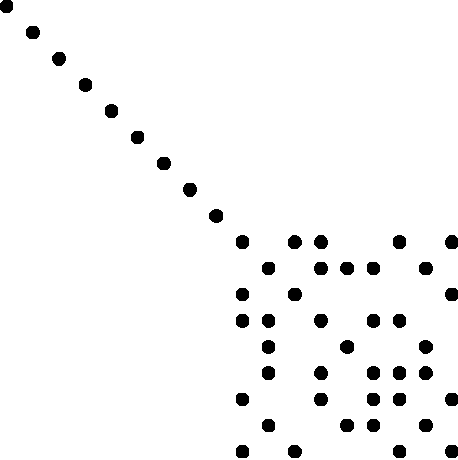
\includegraphics[width=0.25\textwidth]{trap2mat} \, 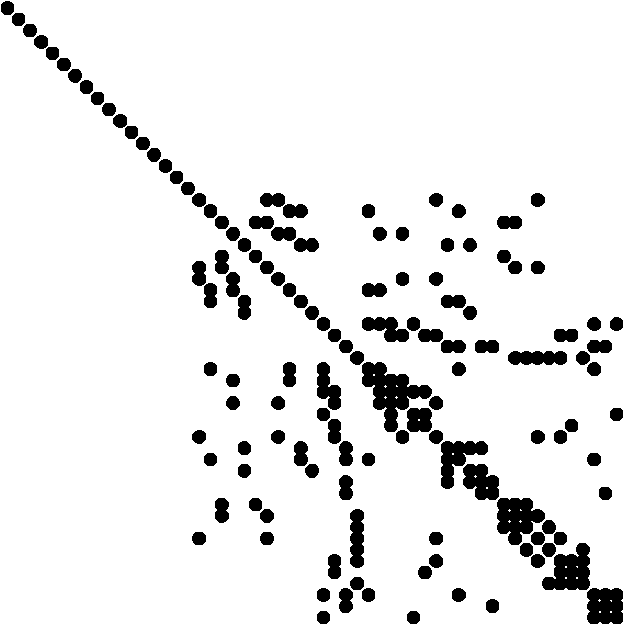
\includegraphics[width=0.25\textwidth]{trapsmat}}

\medskip
\end{itemize}
\end{frame}


\begin{frame}{the Newton step is a sparse linear system}
\begin{itemize}
\item $J_\bF(\bu_k) \bp = - \bF(\bu_k)$ is a sparse linear system
    \begin{itemize}
    \item[$\circ$] solve it for the Newton step $\bp$
    \item[$\circ$] actually take the step after line search: $\bu_{k+1} = \bu_k + \alpha\bp$
    \end{itemize}

\item so, how to solve?:
    $$A \bp = \bb$$

\vspace{-3mm}
    \begin{itemize}
    \item[$\circ$] always: $A=J_\bF(\bu_k)$ is sparse $N\times N$ matrix
    \item[$\circ$] if PDE is well-posed: $A=J_\bF(\bu_k)$ is invertible
    \item[$\circ$] if uniformly elliptic and assembled as described: $A=J_\bF(\bu_k)$ is symmetric positive-definite
    \end{itemize}
\end{itemize}
\end{frame}


\begin{frame}{solving sparse linear systems}
\begin{itemize}
\item the Newton step is $A \bp = \bb$ where $A=J_\bF(\bu_k)$
\item $O(N^3)$ dense algorithms are possible:
    \begin{itemize}
    \item[$\circ$] Gaussian elimination (LU decomposition)
    \item[$\circ$] Cholesky decomposition
    \end{itemize}
\item \dots but they struggle for big $N$
    \begin{itemize}
    \item[$\circ$] variable reordering (minimum degree, nested dissection) helps a lot \dots but is still slow
    \end{itemize}
\item modern expectation: use Krylov methods
    \begin{itemize}
    \item[$\circ$] $\mathcal{K}_m(A,\bb) = \left<\bb,A\bb,A^2\bb,\dots,A^{m-1}\bb\right>$ is \emph{Krylov space}
    \item[$\circ$] CG and GMRES are best-known Krylov methods
    \end{itemize}
\end{itemize}
\end{frame}

\begin{frame}{solving sparse linear systems}
\begin{itemize}
\item actually one uses \emph{preconditioned} Krylov methods
\item a \emph{preconditioner} is an $M$ which is spectrally-equivalent to $A$ and such that $M\bp=\bc$ can be rapidly solved
\item for $A\bp=\bb$ the preconditioned system is $M^{-1} A \bp = M^{-1} \bb$
    \begin{itemize}
    \item[$\circ$] $\mathcal{K}_m(M^{-1} A,M^{-1} \bb)$ contains good approximation of $\bp$
    \end{itemize}
\item preconditioners include:
    \begin{itemize}
    \item[$\circ$] diagonal of $A$ \hfill \emph{Jacobi}
    \item[$\circ$] incomplete factorization \hfill \emph{ILU,IC}
    \item[$\circ$] approximate block inverse \hfill \emph{ASM}
    \item[$\circ$] application of multigrid cycles \hfill \emph{GMG,AMG}
    \end{itemize}
\end{itemize}
\end{frame}


\section{modern software: Python/Firedrake/PETSc}

\begin{frame}{modern FEM software}

\begin{itemize}
\item modern FEM software should make this easy
\item application packages:
    \begin{itemize}
    \item[$\circ$] COMSOL Multiphysics  \hfill $\leftarrow$ grew out of a Matlab toolbox
    \item[$\circ$] ABACUS
    \item[$\circ$] Autodesk Simulation
    \item[$\circ$] I don't actually know much about these \dots
    \end{itemize}
\item open source libraries [language]:
    \begin{itemize}
    \item[$\circ$] deal.II [C++]
    \item[$\circ$] libmesh [C++]
    \item[$\circ$] Elmer [Fortran90]
    \item[$\circ$] FEniCS [Python]
    \item[$\circ$] Firedrake [Python]
    \end{itemize}

\end{itemize}
\end{frame}


\begin{frame}{X}
X
\end{frame}


\begin{frame}{X}
X
\end{frame}


\begin{frame}{X}
X
\end{frame}

\begin{frame}{X}
X
\end{frame}

\begin{frame}{X}
X
\end{frame}

\begin{frame}{X}
X
\end{frame}


\section{runtime choices}

\begin{frame}{X}
X
\end{frame}

\begin{frame}{X}
X
\end{frame}

\begin{frame}{X}
X
\end{frame}

\begin{frame}{X}
X
\end{frame}

\begin{frame}{X}
X
\end{frame}

\begin{frame}{X}
X
\end{frame}


\end{document}
